\documentclass{UoYCSproject}{}
\title{Undecided Title}
\author{Callum Hewitt}
\supervisor{Lilian Blot}
\date{2016 Oct 12}
\wordcount{2}
\BSc
\abstract{
Not completed
}
\dedication{Not completed}
\acknowledgements{
	Not completed
}

\usepackage{listings}
\usepackage{graphicx}
\usepackage{xcolor}
\usepackage{usebib}
\usepackage{tikz}
\usepackage{amsmath}
\usepackage{amssymb}

\bibinput{bibliography}

\newcommand\todo[1]{\emph{{\textcolor{red}{TODO: #1}}}}
\newcommand\newtext[1]{\emph{{\textcolor{blue}{#1}}}}
\newcommand\citetitle[1]{\usebibentry{#1}{title}}

\graphicspath{{images/}}

\usetikzlibrary{shapes,arrows,positioning}
\tikzset{
  font={\fontsize{6pt}{6}\selectfont}
  }
\tikzstyle{startstop} = [rectangle, rounded corners, text centered, draw=black, fill=red!15,text width=2cm]
\tikzstyle{io} = [trapezium, trapezium left angle=70, trapezium right angle=110, text centered, draw=black, fill=blue!15,text width=2cm]
\tikzstyle{process} = [rectangle, text centered, draw=black, fill=orange!15,text width=3cm]
\tikzstyle{decision} = [diamond, aspect=2, text centered, draw=black, fill=green!15,text width=2cm]
\tikzstyle{bigdecision} = [regular polygon, regular polygon sides=6, xscale=3, text centered, draw=black, fill=green!15, text width=5cm]
\tikzstyle{arrow} = [thick,->,>=stealth]


\begin{document}
\maketitle
\listoffigures
\listoftables

\chapter{Introduction}
\label{cha:Introduction}

The terms 'autonomous vehicle' and 'self-driving car' were once thought of as science fiction, but as of recent, they have become our reality. Google's Self-Driving Car Project is gaining traction, with cars currently driving \newtext{in Milton Keynes and }four different US states \citep{GoogleCars}. Tesla Motors have deployed a beta version of their Autopilot system into all of their vehicles produced since September 2014. The system has been blamed for both saving and ending lives \citep{TeslaHospital} \citep{TeslaUnderInvestigation}. 2016 has been a big year for autonomous vehicles and with that comes an even bigger push for robust and secure autonomous systems.
The possible benefits of autonomous vehicles cover a lot of different areas of concern. 

The main issue it addresses is safety. Autonomous vehicles would be able to react to incidents on the road much more quickly than a human driver would. A human's 'thinking distance' can often determine whether someone survives an accident or not. This distance can also be greatly increased if the driver of the vehicles is under the influence of alcohol or narcotics. An autonomous vehicle however, would be able to react to accidents much more quickly than a human, reducing the thinking distance greatly, improving road safety.

\begin{figure}[h]
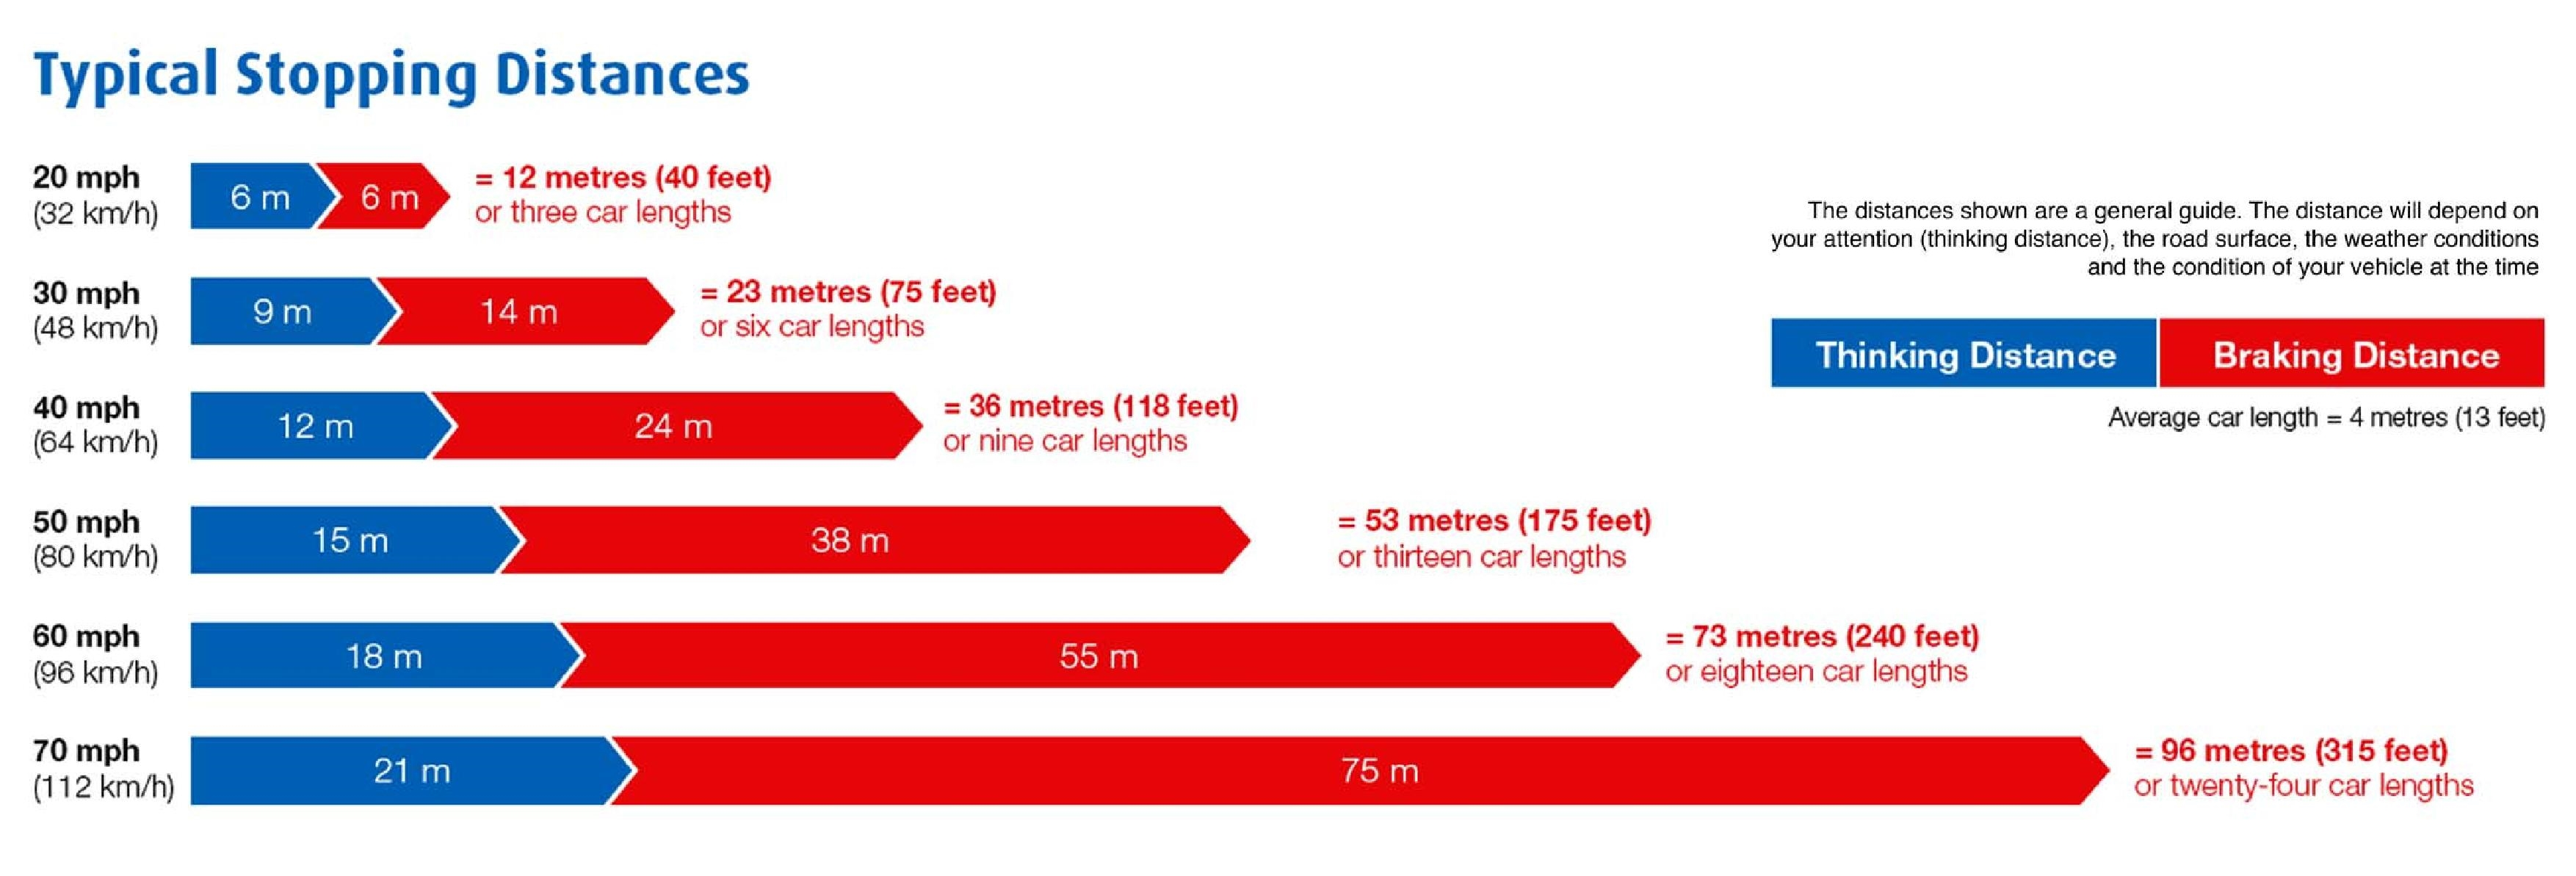
\includegraphics[width=\textwidth]{stoppingDistances.jpg}
\caption{Diagram from Rule 126 in the UK Highway Code \citep{StoppingDistances}}
\end{figure}

Autonomous vehicles could also make transport more efficient. Research by Mersky in April 2016 suggested that fuel conservation control strategies could make autonomous vehicles up to 10\% more fuel efficient than current EPA fuel economy test results \citep{Mersky2016} \todo{Read this article}. Having vehicles which are fuel efficient is becoming increasingly important, with landmark climate change deals such as 'The Paris Agreement' introducing limits on greenhouse gas emissions globally. The introduction of electric vehicles into the car market is also an important factor to consider, as the range of such vehicles still has not managed to match that of their gasoline counterparts. More efficient driving strategies introduced by autonomous vehicles could reduce this gap.

\newtext{Congestion contributes to fuel loss in quite a large way. In the US in 2014 an estimated 3.1 billion gallons (11.7 billion litres) of fuel was wasted due to congestion \citep{Schrank2015}. Automating typical driving activities and communications between vehicles, in situations such as lane changes, could reduce congestion and improve efficiency. Unsafe lane changes don't even have to result in a crash to cause delays. If a car brakes due to a car merging unsafely it can cause a ripple effect, creating a traffic jam.}

Autonomous vehicles also offer a level of comfort not currently available today. In a world where autonomous vehicles are commonplace, it is not hard to imagine people doing work, reading or relaxing in their car instead of having to focus on driving. 

However, today there are still a number of concerns surrounding autonomous vehicles. One of the major concerns is over the reliability of the systems governing the vehicle. These systems need to be responsive and accurate and they cannot afford to fail in such safety critical environments. Already concerns over Tesla's Autopilot system are impacting the image of the company, and the system isn't even out of beta testing yet \citep{TeslaCriticised}. 

In order to address these concerns safely, we can create simulations which test our autonomous systems. These simulations can test the reliability of our systems. Researchers at the University of Texas set up the Autonomous Intersection Management (AIM) project, which aims to " create a scalable, safe, and efficient multiagent framework for managing autonomous vehicles at intersections" \citep{AIMProject}. The project managed to apply their tested intersection software in a mixed reality test using a real life autonomous vehicle \citep{Quinlan2010}, demonstrating how simulations are vital tools when testing these safety critical systems.

\newtext{In this project we make a number of assumptions. Firstly we assume that the sensors resolving the positions of the vehicle and it's surrounding obstacles are perfectly accurate. We also assume that the vehicle can communicate reliably with other vehicles. These assumptions are existing areas of research for autonomous vehicles but are not considered in this paper. The main focus here is on how autonomous vehicles can self-organise to minimise delays in traffic with effective, safe lane merging.}

The aims of this project are as follows:
\begin{itemize}
\item Attempt to generalise the AIM codebase such that other simulations can be created for non-intersection related situations.
\begin{itemize}
\item If the codebase proves difficult to refactor, new simulator code will need to be created
\end{itemize}
\item Use the new codebase to create a decentralised system for managing lane merging.
\item Use the new codebase to create a centralised system for managing lane merging.
\item Compare the effectiveness of both strategies.
\end{itemize}

Creating these simulations helps to determine the effectiveness of two different strategies and also provides a codebase within which future simulations for other situations can be created.
\chapter{Literature Review}
\label{cha:Literature Review}
\newtext{This section. ALL NEW TEXT}

\section{Car Following Models}
\label{sec:Car Following Models}
Most lane changing stem from adjustments made to `Car-Following Models'. These models describe how a vehicle acts based on the actions of the vehicle(s) in front of it. 

One of the early vehicle models was defined by P.G. Gipps in 1981 \citep{Gipps1981}. This model was designed to mimic real-world driver behaviour.

Gipps' 1981 model aims to calculate a safe travel speed based on the vehicle it is following. A safe speed is defined as a speed at which the driver can safely stop in the event that the preceding driver stops.

This is the notation for Gipps' model.

\begin{itemize}
\item[$n-1$] is the vehicle vehicle $n$ is following 
\item[$a_n$] is the maximum acceleration which the driver of vehicle $n$ wishes to undertake.
\item[$b_n$] is the most severe braking that the driver of vehicle $n$ wishes to undertake ($b_n < 0$).
\item[$\hat{b}$] is the vehicle $n$ driver's best guess at $b_{n-1}$
\item[$s_n$] is the effective size of vehicle $n$, that is, the physical length plus a margin into which the following vehicle is not willing to intrude, even when at rest.
\item[$V_n$] is the speed at which the driver of vehicle $n$ wishes to travel.
\item[$x_n(t)$] is the location of the front of vehicle $n$ at time $t$.
\item[$v_n(t)$] is the speed of vehicle $n$ at time $t$.
\item[$\tau$] is the apparent reaction time, a constant for all vehicles.
\end{itemize}

Gipps' paper defines two equations providing constraints on the speed of vehicle $n$ at time $t + \tau$. 

Gipps first defines the acceleration constraint of the vehicle. Essentially this shows that the driver accelerates until they are close to their target speed. The driver then reduces their acceleration until it reaches zero. This equation was obtained through measurements from an instrumented car.

\begin{equation*}
v_n(t+\tau) \leqslant v_n(t) + 2.5a_n\tau\Biggl(\frac{1 - v_n(t)}{V_n}\Biggr)\Biggl(\frac{0.025 + v_n(t)}{V_n}\Biggr)^{1/2}
\end{equation*}

The second constraint is the braking profile of the vehicle. This is given as

\begin{equation*}
\begin{split}
&v_n(t+\tau) \leqslant \\
&b_n\tau + \sqrt{\Biggl(b_n^2\tau^2 - b_n\biggl(2\Bigl[x_{n-1}(t) - s_{n-1} - x_n(t)\Bigr] - v_n(t)\tau - \frac{v_{n-1}(t)^2}{\hat{b}}\biggr)\Biggr)}
\end{split}
\end{equation*}

Therefore, at time $t + \tau$, assuming the driver travels as fast as is safe, and within the limitations of the vehicle, the speed is given by the minimum of these two equations.

One flaw with this model, when it comes to autonomous vehicles, is that it was designed to mimic real-life traffic and all of the problems with human drivers. $\tau$ would be far smaller with an autonomous vehicle. Autonomous vehicles would also be able to better predict the other variables in the constraints including $\hat{b}$, especially when vehicle-to-vehicle communication is possible. Given these more accurate inputs we could construct a model with lower margins for error.

In 2000 Treiber et al. suggested the `Intelligent Driver Model' (IDM). This is the notation for the model

\begin{itemize}
\item[$v_\alpha$] is the velocity of the vehicle $\alpha$
\item[$\dot{v_\alpha}$] is the acceleration of the vehicle $\alpha$
\item[$a^{(\alpha)}$] is the maximum acceleration of the vehicle $\alpha$
\item[$v_0^{(\alpha)}$] is the desired velocity of the vehicle $\alpha$
\item[$\delta$] is the acceleration exponent. Typically 4.
\item[$s_\alpha$] is the gap between vehicle $\alpha$ and the vehicle in front of $\alpha$
\item[$s^*$] is the desired minimum gap between vehicle $\alpha$ and the vehicle in front of $\alpha$
\item[$\Delta v_\alpha$] is the velocity difference, or approaching rate, of vehicle $\alpha$ to the vehicle in front of $\alpha$
\end{itemize}

The acceleration of a vehicle in the Treiber model is a continuous function of the velocity $v_\alpha$, the gap $s_\alpha$ and the approaching rate $\Delta v_\alpha$. Its vehicle interactions are based solely on its relative acceleration to the vehicle in front. It does not provide information about its position, unless it is in relation to the vehicle in front of it, nor does it provide its velocity at a given time, as Gipps' model does. 

It is broken into two components. The first is the action of a vehicle on a free road. The vehicle will accelerate as such

\begin{equation*}
\dot{v_\alpha} = a^{(\alpha)}\Biggl[1 - \biggl(\frac{v_\alpha}{v_0^(\alpha)}\biggr)^\delta\Biggr]
\end{equation*}

The second is the action of a vehicle as it approaches the vehicle in front and needs to decelerate. 

\begin{equation*}
\dot{v_\alpha} = - a^{(\alpha)}\biggl(\frac{s^*}{s_\alpha}\biggr)^2
\end{equation*}

Interpolating these two equations gives us the IDM. 

\begin{equation*}
\dot{v_\alpha} = a^{\alpha}\Biggl[1 - \biggl(\frac{v_\alpha}{v_0^\alpha}\biggr)^\delta - \biggl(\frac{s^*(v_\alpha,\Delta v_\alpha)}{s_\alpha}\biggr)^2\Biggr]
\end{equation*}

Similarly to the Gipps' model the standard IDM only provides a model for one lane. However, unlike Gipps' model it does not attempt to directly mimic human behaviour in traffic situations. It models a general acceleration and braking profile for a given vehicle. As such, it is well suited for adaptation by autonomous vehicle models, as seen in \citep{Kesting2007}.

\todo{Think about more comparisons - Talk to Lilian.}
\todo{Possibly include the PlatooningAV paper in here \citep{Kamali2016}}

\section{Centralised Systems}
\label{sec:Centralised Systems}
We can generally divide approaches to autonomous vehicles into centralised solutions and decentralised solutions. Centralised solutions rely on an external agent to manage the AVs. The AVs use vehicle-to-infrastructure (V2I) communication channels to send information and receive instructions from the external agent. Decentralised solutions use vehicle-to-vehicle (V2V) communication to let other vehicles know their state, their intentions and to arrange any complex actions that might affect surrounding vehicles.

The Autonomous Vehicle Intersection management system (AIM) described in \citep{Dresner2004} is an example of a centralised V2I system. The system works by dividing the intersection into a grid of $n \times n$ reservation tiles. Drivers `call ahead' to the intersection sending information about

\begin{enumerate}
\item The time the vehicle will arrive.
\item The velocity at which the vehicle will arrive
\item The direction the vehicle will be facing when it arrives
\item The vehicle's maximum velocity
\item The vehicle's maximum and minimum acceleration
\item The vehicle's length and width
\end{enumerate}

The intersection infrastructure simulates the journey of the vehicle through the intersection noting the tiles occupied by the vehicle at each time interval. If any cell is reserved at the same time step the intersection rejects the request. The driver will start decelerating and continue making requests until it obtains a reservation. It will not enter the intersection without a reservation, even if that means decelerating to a stop.

\todo{Insert image of aim here.}

A grid-based reservation system works well in high traffic zones like intersections because it forces all vehicles to communicate with a single entity. This achieves a global-view of activity at that junction making it much easier to manage. A V2V solution would require complex communication protocols, possibly with large numbers of vehicles.

However, using a centralised system does create a single point of failure. If the system fails it could lead to collisions in the intersection with the AVs having no way to determine whether it is safe to enter or not. A V2V system would be more fault tolerant, with vehicles being able to navigate their way through a system by themselves.

A centralised system for lane changing was described in a paper by Atagoziyev et al. in 2016 \citep{Atagoziyev2016}. This system uses roadside infrastructure to help groups of vehicles change lanes before they reach a `critical-position'. These critical-positions could be areas such as motorway exits or intersections.

The vehicles send their position and velocity information to the roadside infrastructure and the system then sends a number of orders to the vehicles such that they safely rearrange themselves into the correct lanes. 

Because the distances involved can be large, particularly at high speeds, the system would struggle to use a reservation tile based system as AIM did, instead it manages the gaps between vehicles to safely relocate vehicles into the correct positions. A more comprehensive overview is given in \ref{subsec:Lane Changing to hit a target lane}.

This system again works very well here because critical points will tend to be high traffic areas so it helps to deal with the issue of large volumes of V2V communications. It also falls into the same pitfall of being a single point of failure. In fact you could argue that for situations such as motorway exits, the consequences of failure are much more severe.

\section{Making lane changing decisions}
\label{sec:Making lane changing decisions}
There are a number of reasons that a driver would want to change lanes. The most obvious being that the overall journey the driver wishes to complete requires the vehicle to move into a different lane. In this case the vehicle \emph{must} change lanes before a `critical point'. Beyond this point the driver will need to change their planned route, most likely extending their journey time. 

Another reason a driver might change lanes is in order to increase velocity, with the aim of reducing journey time. In general, a driver will aim to change lanes if their average velocity in their current lane is much less than that the velocity it could be achieving in another lane.

\subsection{Lane Changing to hit a target lane}
\label{subsec:Lane Changing to hit a target lane}
In 1986 Gipps' modelled driver behaviour in real world circumstances, characterising the decisions a driver has to make in order to determine whether to change lanes. The paper was designed to be used with the Gipps' 1981 car-following model \citep{Gipps1981}, explained in \ref{sec:Car Following Models}.

The model itself is constructed as a flow chart, in which the decision nodes are the choices a driver must make. 

\todo{Create flowchart figure}

After determining whether a lane change is feasible the model considers whether the driver needs to move into another lane because they are heading towards a critical point.

These decisions are modelled in nodes 3 and 4.

\begin{enumerate}
\item[3] \textit{Driver behaviour close to the intended turn}

If the driver is close to their intended turn then they will always attempt to change into their preferred lane. Only if blocked will they consider moving into another lane. 

`Close' varies depending on regional differences and the level of traffic, but in the model, close is defined as the driver being within a distance equal to ten seconds of travel from the turn at the driver's desired speed.

\item[4] \textit{Urgency of changing lanes}

The urgency of changing lanes increases as the driver gets closer to their turn. The willingness of the driver to brake harder and accept smaller gaps increases as the driver gets closer to their intended turn.

In the implementation, the braking rate a driver is willing to when first becoming close doubles by the time the intended turn is reached. 

\begin{itemize}
\item[$D_n$] is the location of the intended turn
\item[$V_n$] is the desired (or free) speed of the driver
\item[$b_n^*$] is the most severe braking the driver would otherwise be willing to undertake
\end{itemize}

\begin{equation*}
b_n = \Biggl[2 - V_n\frac{(D_n - x_n(t))}{10}\Biggr]b_n^*
\end{equation*}

\end{enumerate}

This driver decision model is useful, and a good example of a decentralised system. Each driver's decisions are made without a global view of all other drivers. The driver simply adjusts their behaviour as they approach their turn. This provides a fault tolerant solution to the problem, where one vehicle can compensate for the failings of another. However, this does leave the system open to failures due to poor organisation between vehicles. 

Atagoziyev et al. method forces vehicles to work together to manage lane changes before the critical point. The notation for the Atagoziyev model is

\begin{itemize}
\item Vehicles and Points
\begin{itemize}
\item[CP] is the critical point
\item[SV] is the subject vehicle. The vehicle making a lane change.
\item[CL] is the vehicle in front of the SV in the SV's current lane.
\item[TL] is the vehicle in front of the SV in the target lane.
\item[LV] is the lag vehicle behind SV in the target lane.
\end{itemize}
\item Positions
\begin{itemize}
\item[$x$] is the unknown position of SV
\item[$x_l$] is the unknown position of LV
\item[$x_{cl}$] is the trajectory of CL
\item[$x_{tl}$] is the trajectory of TL
\item[$x(t)$] is the position of SV at time $t$
\item[$x_{cl}(t)$] is the position of CL at time $t$
\item[$x_{tl}(t)$] is the position of TL at time $t$
\item[$x_l(t)$] is the position of LV at time $t$
\item[$x_{clb}$] is the CL bound. SV must be located behind this bound during the lane change.
\item[$x_{tlb}$] is the TL bound. SV must be located behind this bound during the lane change.
\item[$x_{lb}$] is the LV bound. SV must be located in front of this bound during the lane change.
\item[$x_{min}(t)$] is the minimum of $x_{tlb}$ and $x_{clb}$ at time $t$
\end{itemize}
\item Times
\begin{itemize}
\item[$t_{end}$] is the available time until the `string leader' reaches the critical point. The string is the set of cars involved in changing lanes.
\item[$0,t_{end}$] is the time interval available for the lane change manoeuvre.
\item[$\hat{t}$] is the earliest possible time a lane change of SV can be performed.
\item[$\Delta_{LC}$] is the time taken to change lanes.
\item[$W$] is the set of time windows where the leader vehicles enabled a lane change. It is given as 
\begin{equation*}
W = {[t_1,t_2]|t_2 \ge t_1 + \Delta_{LC} \land v_{cl}(t) = v_{tl}(t) = v_{nom} \forall t \in [t_1,t_2]}
\end{equation*}
\end{itemize}
\item Velocities
\begin{itemize}
\item[$v_{nom}$] is the nominal speed of the vehicles.
\item[$v_{up}$] is faster than average velocity.
\item[$v_{dn}$] is slow than average velocity.
\item[$v_{cl}$] is the CL velocity.
\item[$v_{tl}$] is the TL velocity.
\item[$v_{min}(t)$] is the minimum of $v_{tlb}$ and $v_{clb}$ at time $t$
\end{itemize}
\end{itemize}

The Atagoziyev model performs a number of lane changes in order to rearrange the vehicles into the right lanes. To do this it loops through all of the vehicles that aren't in the right lane.

\todo{Explain all of the Atagoziyev model? It seems excessive.}

\subsection{Lane Changing to improve overall velocity}
\label{subsec:Lane Changing to improve overall velocity}
Gipps' driver decisions model also considered situations where the driver does not have to be in any particular lane. The model considers the effects of transit lanes, heavy vehicles and the effect of the preceding vehicle on the driver's vehicle. These are shown in nodes 5 to 7 and 9 to 11.

\begin{enumerate}
\item[5] \textit{Transit vehicles and lanes}
Transit lanes are lanes dedicated solely for public transport and other high occupancy vehicles. These include vehicles such as buses, taxis and carpool cars. These vehicles are known in the model as `transit vehicles'.
\item[6] \textit{Entry of nontransit vehicles into transit lanes}
If there is an obstruction in the present lane, it is often considered to be a valid reason for a non-transit vehicle to enter a transit lane. 
\item[7] \textit{Departure of nontransit vehicles from a transit lane}
Once the obstruction has been cleared, nontransit vehicle must move back into a valid lane. This forced departure does not affect vehicles that are close to their intended turn.
\item[9] \textit{Relative advantages of present and target lanes}
If the driver has not yet been forced to change lanes by any other factors, then they can look at the relative advantages of the present and target lanes, considering obstructions and then determining which lanes obstructions will have the least effect on their safe speed.
\item[10] \textit{The effect of heavy vehicles} 
If obstructions are level with each other or beyond the range a driver considers, then the driver considers the next heavy vehicle in each lane, as if it were the leading vehicle in an ordinary car following situation. The driver then selects the lane which will give them the higher speed.
\item[11] \textit{The effect of the preceding vehicle}
If there are then no heavy vehicles, the driver considers the speed possible in each lane and then changes if they gain a `sufficient' speed advantage. This is again, subjective, depending on the present lane, target lane and the type of vehicle.
\end{enumerate}

In areas where traffic is flowing quickly and there aren't a large number of vehicles to organise around, decentralised models like this work very well. Vehicles can act independently of each other fairly easily. However, Gipps' model is based on human interaction and does not consider the global effect of a lane change. The work by Kesting et al. in 2007 \citep{Kesting2007} produces a decentralised model for lane changes which also considers the effect of your lane change on other vehicles. This can help to reduce the `phantom intersection' effect and improve overall traffic flow.

\todo{Explain what Kesting did and compare it to Gipps' model.}
\chapter{Implementation}
\label{cha:Implementation}
The final implementation was done in Java, an was built on top of the AIM simulator codebase. All class diagrams were created using IntelliJ IDEA 15.0.3 internal diagram tool. Figure \ref{fig:classDiagramKey} provides a key for understanding these diagrams.

\section{Generalising the Codebase}
\label{sec:Generalising the Codebase}
\begin{tabular}{|c|c|c|}
\hline
Requirement Code & Acheived? \\
\hline
NS.11 & \cellcolor{green} \cmark \\
NS.12 & \cellcolor{green} \cmark \\ 
\hline
\end{tabular}

The use of the AIM codebase was a project restriction imposed for research purposes. By working with the AIM simulator codebase I could learn how easy it is to work with, and analyse whether or not it will be a good codebase to continue expanding upon for future AV projects. Each simulator built for this project works alongside the AIM simulators, whilst being completely independent. The project: 'A self-organising approach to autonomous vehicle car park management using a message-based protocol' \citep{Milligan2017}, also uses simulators built using AIM. To make sure that code coupling was reduced as much as possible, I worked closely with their project lead to generalise the codebase, breaking out useful shared features so that they could be accessed by all simulator types.

\begin{figure}[htb]
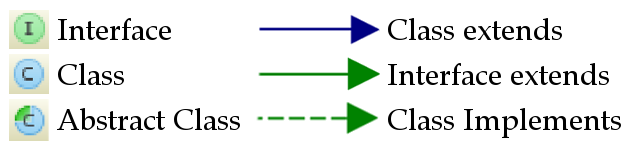
\includegraphics[width=\textwidth]{classDiagrams/classDiagramKey.png}
\caption{Key for the class diagrams in this report.}
\label{fig:classDiagramKey}
\end{figure}

\todo{Decide what to put here} Appendix \ref{sec:Generalising the Codebase Appendix} provides detailed coverage of both this change, and changes made to some of the other areas of the AIM codebase.

\section{Merge Schemes}
\label{sec:Merge Schemes}
\begin{tabular}{|c|c|c|}
\hline
Requirement Code & Acheived? \\
\hline
FS.81 & \cellcolor{red} \xmark \\
FS.91 & \cellcolor{red} \xmark \\
\hline
\end{tabular}
The original plan was to implement two merge schemes, an AIM based centralised protocol and a dentralised approach based on \citetitle{VanMiddlesworth2008} \citep{VanMiddlesworth2008}. However, implementation proved to be very difficult. 

The AIM protocol implementation was developed by examining the original AIM code and creating a modified version applicable to merges. Because the two systems are so similar, much of the code was duplicated. This could be refactored out a later date, but during development having full control over the actions taken by a vehicle without having to compromise to allow AIM to work correctly was very useful. In the end, despite this approach there were significant issues with the system. Despite using very similar approaches to AIM, almost identical in areas, vehicles would continue to arrive early to their reserved times and vehicles would also collide consistently at intersections.

The system also suffered from some more fundamental problems. Reservations for merges are only taken by the lead vehicle in each lane, as vehicles behind them shouldn't be able to reserve ahead of the lead vehicle. This leads to slow downs at the merge zone as secondary vehicles won't be able to make reservations until the lead vehicle has entered the merge. If secondary vehicles also have to compete with vehicles on the other lane then it is likely that at least one of them will have to stop at the merge. This is fine for four-way stops, but for a merge where maintaining vehicle flow is the primary aim, this system will be far less effective.

The AIM protocol also fails to ensure that one lane does not suffer for the benefit of the other. Reservations are granted on a first-come-first-serve basis (though this could be changed by implementing a different reservation policy) and this can lead to long periods of time where one lane fails to make reservations whilst the other passes vehicles through quickly. Again, this fails to maintain traffic flow, one of the key aims of a merging protocol.

- Queue
As a response to AIM, I developed an alternative centralised approach to the merge problem. Described in 

-- Response to AIM's failings
-- Describe how it was implemented

- Decentralised
-- Never implemented due to time constraints.

\section{Simulation}
\label{sec:Simulation}
\begin{tabular}{|c|c|c|}
\hline
Requirement Code & Acheived? \\
\hline
FS.12 & \cellcolor{green} \cmark \\
FS.13 & \cellcolor{green} \cmark \\
FS.22 & \cellcolor{green} \cmark \\
FS.32 & \cellcolor{green} \cmark \\
FS.42 & \cellcolor{green} \cmark \\
FS.71 & \cellcolor{green} \cmark \\
FS.73 & \cellcolor{green} \cmark \\
FS.172 & \cellcolor{red} \xmark \\
NS.3 & \cellcolor{green} \cmark \\
NS.4 & \cellcolor{green} \cmark \\
NS.8 & \cellcolor{green} \cmark \\
\hline
\end{tabular}

Each simulation consists of multiple interacting agents, which makes it a difficult problem to implement. Using some of the generalised AIM classes helped to reduce the amount of time it took to implement these components. However, using AIM did introduce some complications and parts of the code had to be rewritten to adjust for this.

\subsection{Drivers}
\label{subsec:Drivers}
Driver agents are responsible for manipulating the vehicles in the simulation. They make requests to centralised merge managers and act upon the responses they are given. Each driver acts as a finite state machine, performing specific sets of actions for each state. Vehicles and Drivers both extend from generalised Vehicle and Driver classes containing useful functions for following lanes, turning and determining distances. However, some of these methods proved to be flawed.

One of the main issues was the assumption that lanes and roads will always meet at 90\degree. This caused a number of small issues throughout development, but one key problem was turning. A turn through an intersection in the AIM simulator is done by forcing the vehicle to point to a coordinate further down the lane the vehicle is following. This point is always exactly the same distance away from the vehicle, such that when the vehicle reaches a corner, and the lane it's following changes, the vehicle will turn towards that point gradually. This distance proved too much for some merges, and resulted in the vehicle making turns too gradually. This was fixed by setting the turn distance to always be the distance from the point at which the vehicle enters the merge zone, to the merge zone exit. The target point would also always lie in the centre of the target lane. This caused merging vehicles to turn more tightly, freeing up the lane for more vehicles. Figure \ref{fig:turning} shows how these turns work.

\begin{figure}[htb]
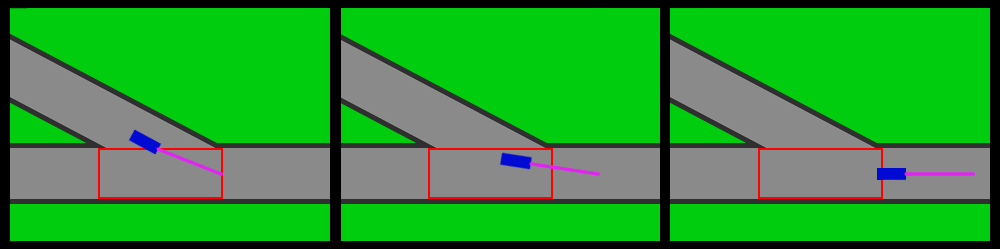
\includegraphics[width=\textwidth]{implementationDiagrams/turning.png}
\caption{Key for the class diagrams in this report.}
\label{fig:turning}
\end{figure}

Another problem came about due to collisions. AIM had provided a method called \emph{dontHitCarInFront} which calculates the distance from the vehicle to the vehicle in front and then takes action to avoid a collision, slowing down if necessary. This method turns out to not be completely effective. Even within the AIM simulations vehicles are colliding. Due to time constraints collision detection was removed from the project as I did not have time to go hunting for the error causing collisions. Overall it does not matter too much as the cars only collide momentarily before separating, but it does make it difficult to detect collision errors caused by merging algorithms. As far as I can tell, no collisions take place with the algorithm implemented, as it should be almost imposible, but without having a check in place this cannot be said for certain.

\subsection{Merge Managers}
\label{subsec:Merge Managers}
The role of a merge manager is to take requests from drivers and provide responses, controlling the flow of traffic through the merge zone. They were heavily influenced by the approaches taken by AIM. The AIM based merge manager replicated much of the intersection manager code introduced by AIM. At a later date this could be refactored to reduce duplication, but this would most likely also require changes to Driver and Vehicle, as each type of merge manager deals with different types of vehicles and drivers.

The final implementation of a merge manager, the QueueV2IManager, is designed similarly to AIM's V2IIntersectionManager, however much of the technical code is original and far simpler. This merge manager effectively just manages a queue and alerts vehicles when they are at the front of said queue. The AIM system is more complex, requiring the merge manager to monitor reservations and time the arrival of vehicles as they arrive. The AIM system relies very heavily on each vehicle arriving at their stated time and fails to handle vehicles well if they don't.

\subsection{Map}
\label{subsec:Map}
The simulation map stores all of the spawn points, lanes and merge managers for the simulation. The calcualtions for lane positions and spawn points were created using the designs in \ref{sec:Map}. 

By using some of the generalised components for calculating distances, creating the map was relatively straightforward, however, there were some components that failed to work as intended. The original AIM system assumes that every road meets at 90\degree and as such some methods were inappropriate for when lanes meet at other angles. One example of this is the no vehicle zone at the beginning of each lane. This zone stops multiple vehicles from spawning on top of each other. The original implementation calculated a Rectangle at the beginning of each lane, which works fine when lanes are at 90\degree. For my no vehicle zones, I had to draw a path around the start of each merge lane and create a shape from that. This more complicated approach was necessary due to the angles at which the merge lane can meet the target lane. 

The map also controls the spawn points creating the vehicles. Most spawning behaviours were based on the AIM spawn points. However, to enable consistent testing we wanted to be able to repeat the experiment with the same vehicles over and over again. To do this I created a new vehicle spawn type that uses a JSON file to spawn vehicles. The file contains a vehicle specification and a time. The spawner reads this data in and spawns a vehicle with the given specification at the indicated time. I also implemented this type of spawner into the AIM system. This means that comparisons between the performance of AIM and the Queue protocol are now possible.

\subsection{Simulation Control}
\label{subsec:Simulation Control}
The simulator itself is reponsible for triggering and monitoring the actions of each component of the simulation. It delivers messages between merge managers and vehicles and moves vehicles through the simulation according to their specified velocities and headings.

\section{Results Production}
\label{sec:Results Production}
\begin{tabular}{|c|c|c|}
\hline
Requirement Code & Acheived? \\
\hline
FS.62 & \cellcolor{green} \cmark \\
FS.63 & \cellcolor{green} \cmark \\
FS.64 & \cellcolor{green} \cmark \\
FS.65 & \cellcolor{green} \cmark \\
FS.66 & \cellcolor{red} \xmark \\
FS.67 & \cellcolor{red} \xmark \\
FS.68 & \cellcolor{green} \cmark \\
FS.69 & \cellcolor{red} \xmark \\
FS.6a & \cellcolor{red} \xmark \\
NS.7 & \cellcolor{green} \cmark \\
\hline
\end{tabular}
- Results generation to CSV file
- Drivers, spawners and simulations adapted to provide the relevant export information
- Setup in AIM as well
- Whay wasn't max accell stored?

\section{GUI}
\label{sec:GUI}
\begin{tabular}{|c|c|c|}
\hline
Requirement Code & Acheived? \\
\hline
FS.11 & \cellcolor{green} \cmark \\
FS.21 & \cellcolor{green} \cmark \\
FS.31 & \cellcolor{green} \cmark \\
FS.41 & \cellcolor{green} \cmark \\
FS.51 & \cellcolor{green} \cmark \\
FS.61 & \cellcolor{green} \cmark \\
FS.72 & \cellcolor{green} \cmark \\
FS.82 & \cellcolor{red} \xmark \\
FS.92 & \cellcolor{red} \xmark \\
FS.101 & \cellcolor{green} \cmark \\
FS.111 & \cellcolor{green} \cmark \\
FS.121 & \cellcolor{green} \cmark \\
FS.131 & \cellcolor{green} \cmark \\
FS.141 & \cellcolor{green} \cmark \\
FS.151 & \cellcolor{green} \cmark \\
FS.161 & \cellcolor{green} \cmark \\
FS.171 & \cellcolor{red} \xmark \\
NS.1 & \cellcolor{green} \cmark \\
NS.2 & \cellcolor{green} \cmark \\
NS.5 & \cellcolor{green} \cmark \\
NS.6 & \cellcolor{green} \cmark \\
\hline
\end{tabular}

The GUI for the project was built using Java Swing, extending the existing AIM GUI. New simulator types are given a separate tab in the application with their own simulator setup and a display screen. The display screen can be modified for each simulation type, showing the relevant information for that simulation. We moved away from the AIM full illustrated canvas implementation to a 'StatScreen' implementation which shows information in text format instead. The S2S simulations display the current simulation time, number of completed vehicles and throughput. They also display two tables, one containing information about the vehicles currently in the simulation, and another for vehicles that have left the simulation. Figure \ref{fig:s2sSimScreen} shows the simulation screen for S2S merges.

-- Consistent testing upload 

\begin{figure}[htb]
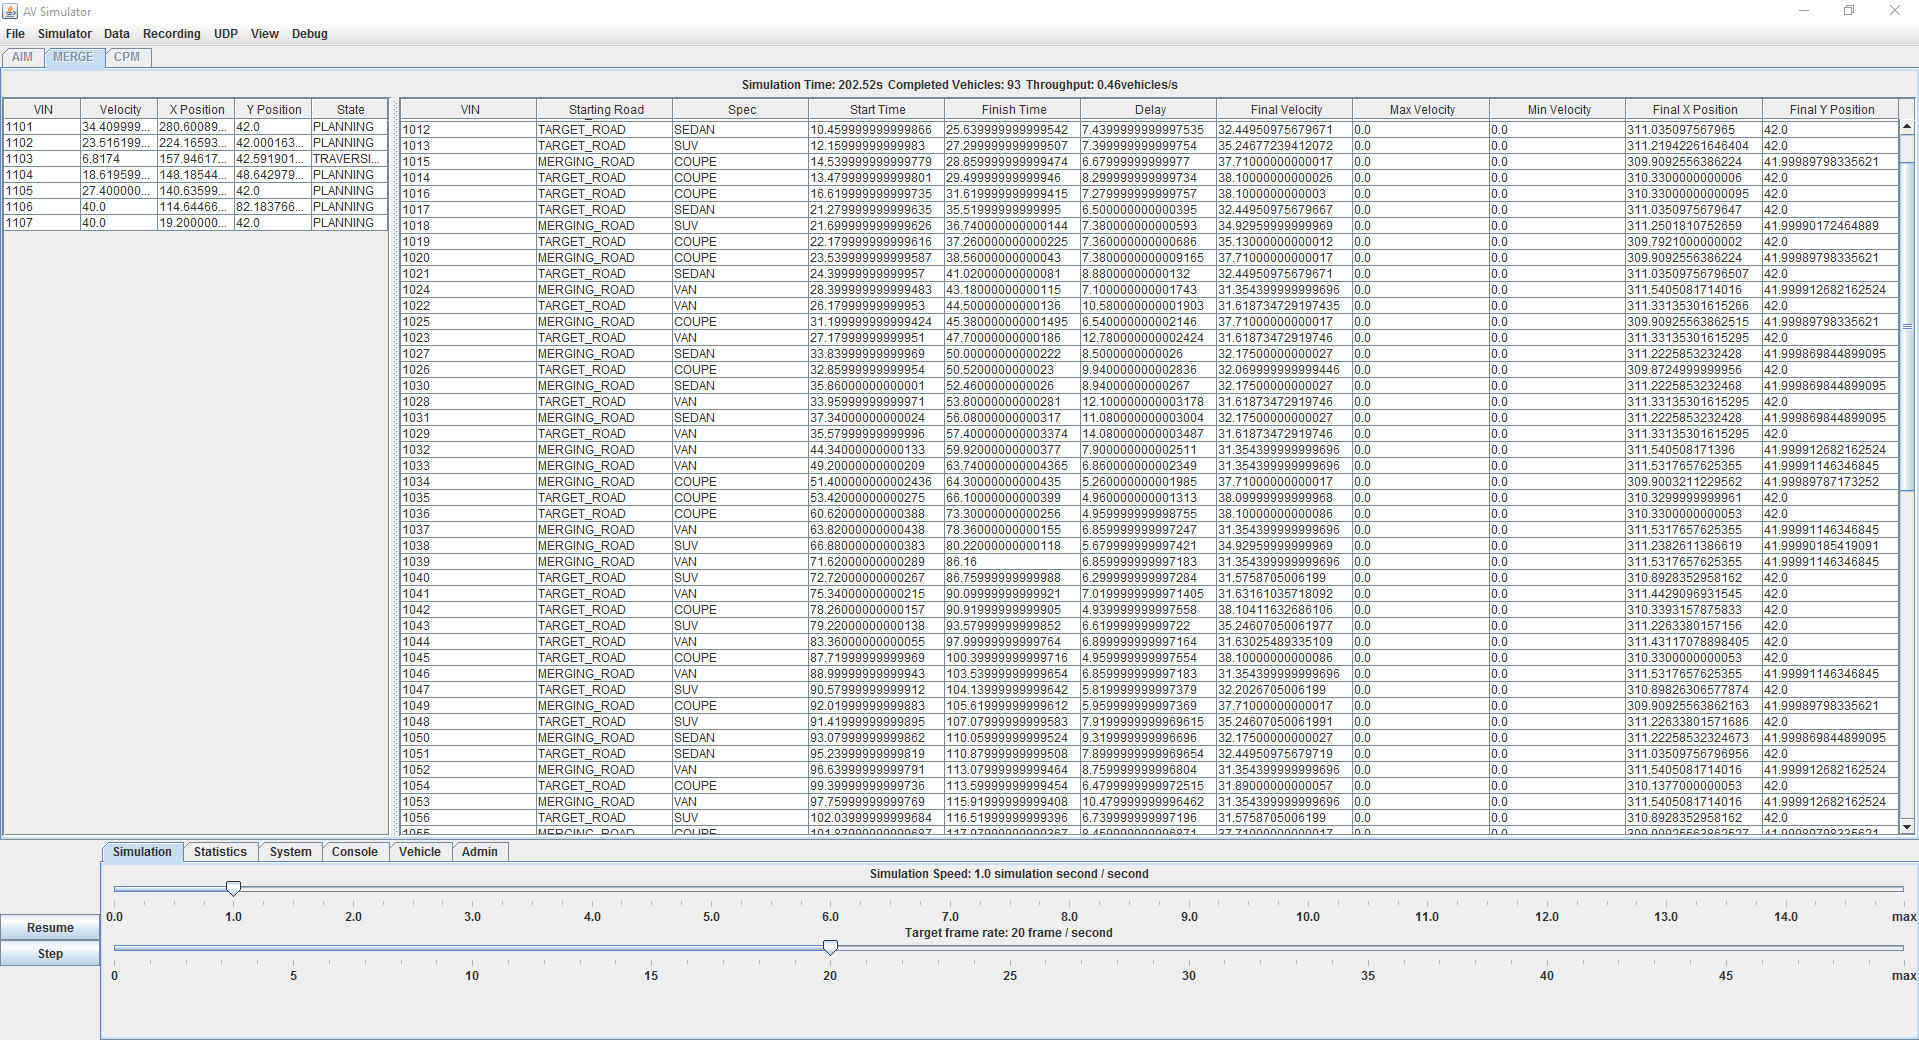
\includegraphics[width=\textwidth]{screenshots/s2sSimulationScreen.png}
\caption{The simulation screen for the S2S merge screen}
\label{fig:s2sSimScreen}
\end{figure}

Functional requirements \emph{FS.82} and \emph{FS.92} were not fully implemented as the AIM-like simulations and Decentralised simulations were never implemented in a fully working form. \emph{FS.171} was also never implemented due to the removal of collision detection from simulations. All other GUI requirements were completed.

\section{Maintainability and Testing}
\label{sec:Testing}
\begin{tabular}{|c|c|c|}
\hline
Requirement Code & Acheived? \\
\hline
NS.9 & \cellcolor{green} \cmark \\
NS.10 & \cellcolor{green} \cmark \\
\hline
\end{tabular}

\subsection{Unit Testing}
\label{subsec:Unit Testing}
Unit tests were mostly used to ensure getter and setter methods worked as expected. However, some unit tests were used to verify the behaviour of classes. To do this I used Mockito \citep{MockitoWebsite} to mock the behaviour of objects used by the test class so that I could prompt the test class into producing the expected results.

\subsection{Integration Tests}
\label{subsec:Integration Tests}



\bibliography{bibliography}{}

\end{document}